%%%%%%%%%%%%%%%%%%%%%%%%%%%%%%%%%%%%%%%%%
% Beamer Presentation
% LaTeX Template
% Version 1.0 (10/11/12)
%
% This template has been downloaded from:
% http://www.LaTeXTemplates.com
%
% License:
% CC BY-NC-SA 3.0 (http://creativecommons.org/licenses/by-nc-sa/3.0/)
%
%%%%%%%%%%%%%%%%%%%%%%%%%%%%%%%%%%%%%%%%%

%----------------------------------------------------------------------------------------
%	PACKAGES AND THEMES
%----------------------------------------------------------------------------------------

\documentclass{beamer}
\usepackage{amssymb}
\usepackage{mathpazo}
\usepackage{media9}
\usepackage{graphicx}
\usepackage{animate}
\usepackage{charter}
\mode<presentation> {

% The Beamer class comes with a number of default slide themes
% which change the colors and layouts of slides. Below this is a list
% of all the themes, uncomment each in turn to see what they look like.

%\usetheme{default}
%\usetheme{AnnArbor}
%\usetheme{Antibes}
%\usetheme{Bergen}
%\usetheme{Berkeley}
%\usetheme{Berlin}
%\usetheme{Boadilla}
\usetheme{CambridgeUS}
%\usetheme{Copenhagen}
%\usetheme{Darmstadt}
%\usetheme{Dresden}
%\usetheme{Frankfurt}
%\usetheme{Goettingen}
%\usetheme{Hannover}
%\usetheme{Ilmenau}
%\usetheme{JuanLesPins}
%\usetheme{Luebeck}
%\usetheme{Madrid}
%\usetheme{Malmoe}
%\usetheme{Marburg}
%\usetheme{Montpellier}
%\usetheme{PaloAlto}
%\usetheme{Pittsburgh}
%\usetheme{Rochester}
%\usetheme{Singapore}
%\usetheme{Szeged}
%\usetheme{Warsaw}

% As well as themes, the Beamer class has a number of color themes
% for any slide theme. Uncomment each of these in turn to see how it
% changes the colors of your current slide theme.

%\usecolortheme{albatross}
%\usecolortheme{beaver}
%\usecolortheme{beetle}
%\usecolortheme{crane}
%\usecolortheme{dolphin}
%\usecolortheme{dove}
%\usecolortheme{fly}
%\usecolortheme{lily}
%\usecolortheme{orchid}
%\usecolortheme{rose}
%\usecolortheme{seagull}
%\usecolortheme{seahorse}
%\usecolortheme{whale}
%\usecolortheme{wolverine}

%\setbeamertemplate{footline} % To remove the footer line in all slides uncomment this line
%\setbeamertemplate{footline}[page number] % To replace the footer line in all slides with a simple slide count uncomment this line

%\setbeamertemplate{navigation symbols}{} % To remove the navigation symbols from the bottom of all slides uncomment this line
}
\def\Xint#1{\mathchoice
{\XXint\displaystyle\textstyle{#1}}%
{\XXint\textstyle\scriptstyle{#1}}%
{\XXint\scriptstyle\scriptscriptstyle{#1}}%
{\XXint\scriptscriptstyle\scriptscriptstyle{#1}}%
\!\int}
\def\XXint#1#2#3{{\setbox0=\hbox{$#1{#2#3}{\int}$ }
\vcenter{\hbox{$#2#3$ }}\kern-.6\wd0}}
\def\ddashint{\Xint=}
\def\dashint{\Xint-}
\usepackage{graphicx} % Allows including images
\usepackage{booktabs} % Allows the use of \toprule, \midrule and \bottomrule in tables
\mode<presentation>{}
%----------------------------------------------------------------------------------------
%	TITLE PAGE
%----------------------------------------------------------------------------------------

\title[prediction and learning]{Text Classification and Multitask Learning} % The short title appears at the bottom of every slide, the full title is only on the title page

\author{Hong Zhang} % Your name
\institute[Yahoo!] % Your institution as it will appear on the bottom of every slide, may be shorthand to save space
{
Yahoo Researh \\ % Your institution for the title page
\medskip
}
\date{\today} % Date, can be changed to a custom date

\begin{document}

\begin{frame}
\titlepage
\end{frame}
\begin{frame}
\tableofcontents
\end{frame}

\section{Text Classification}
\begin{frame}
\begin{itemize}
\item Text classification is a classical topics in Natural Language Processes, e.g., spam filtering,
sentiment analysis,  DA, RA, intent models, \ldots
\item Two components: Sentence representation and classification 
\end{itemize}
\end{frame}



\begin{frame}
\frametitle{Sentence embedding}
Traditional Methods:
\begin{itemize}
\item Bag of words and its TFIDF (term frequency-inverse document frequency)
\item Bag of ngrams and its TFIDF
\end{itemize}
Deep Learning:
\begin{itemize}
\item Word-based ConvNets
\item Character-based ConvNets
\item {\textit{LSTM}} 
\end{itemize}

\end{frame}


\begin{frame}
\frametitle{LSTM}
\begin{figure}
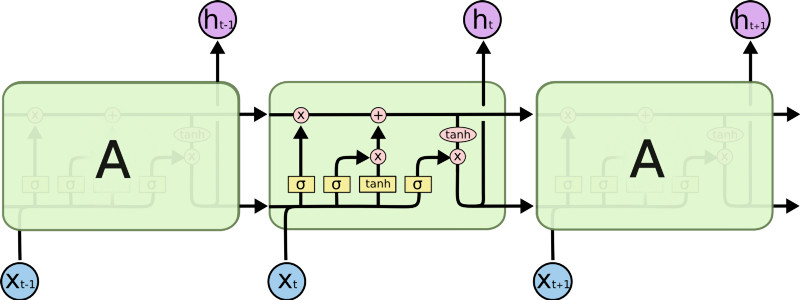
\includegraphics[scale = 0.3]{LSTM.jpg}
\end{figure}
\begin{itemize}
\item \textit{Use the last state as the sentence representation} 
\item Use the average of the states as the representation (not yet implemented)
\end{itemize}

\end{frame}






\section{Regularization Techniques}
\frame{\tableofcontents[currentsection]}
\begin{frame}
\frametitle{Regularizations}
DA-movie has 8.5k training data and 1k validation data.  The dimension of Glove embedding is 300 and hidden state's dimension is 256. Overfitting is an obvious problem. 
Standard regularization techniques: 
\begin{itemize}
\item early stop
\item label smoothing
\item ridge/lasso
\item multitask learning

\end{itemize}


\end{frame}




\begin{frame}
\frametitle{multitask learning}
\begin{figure}
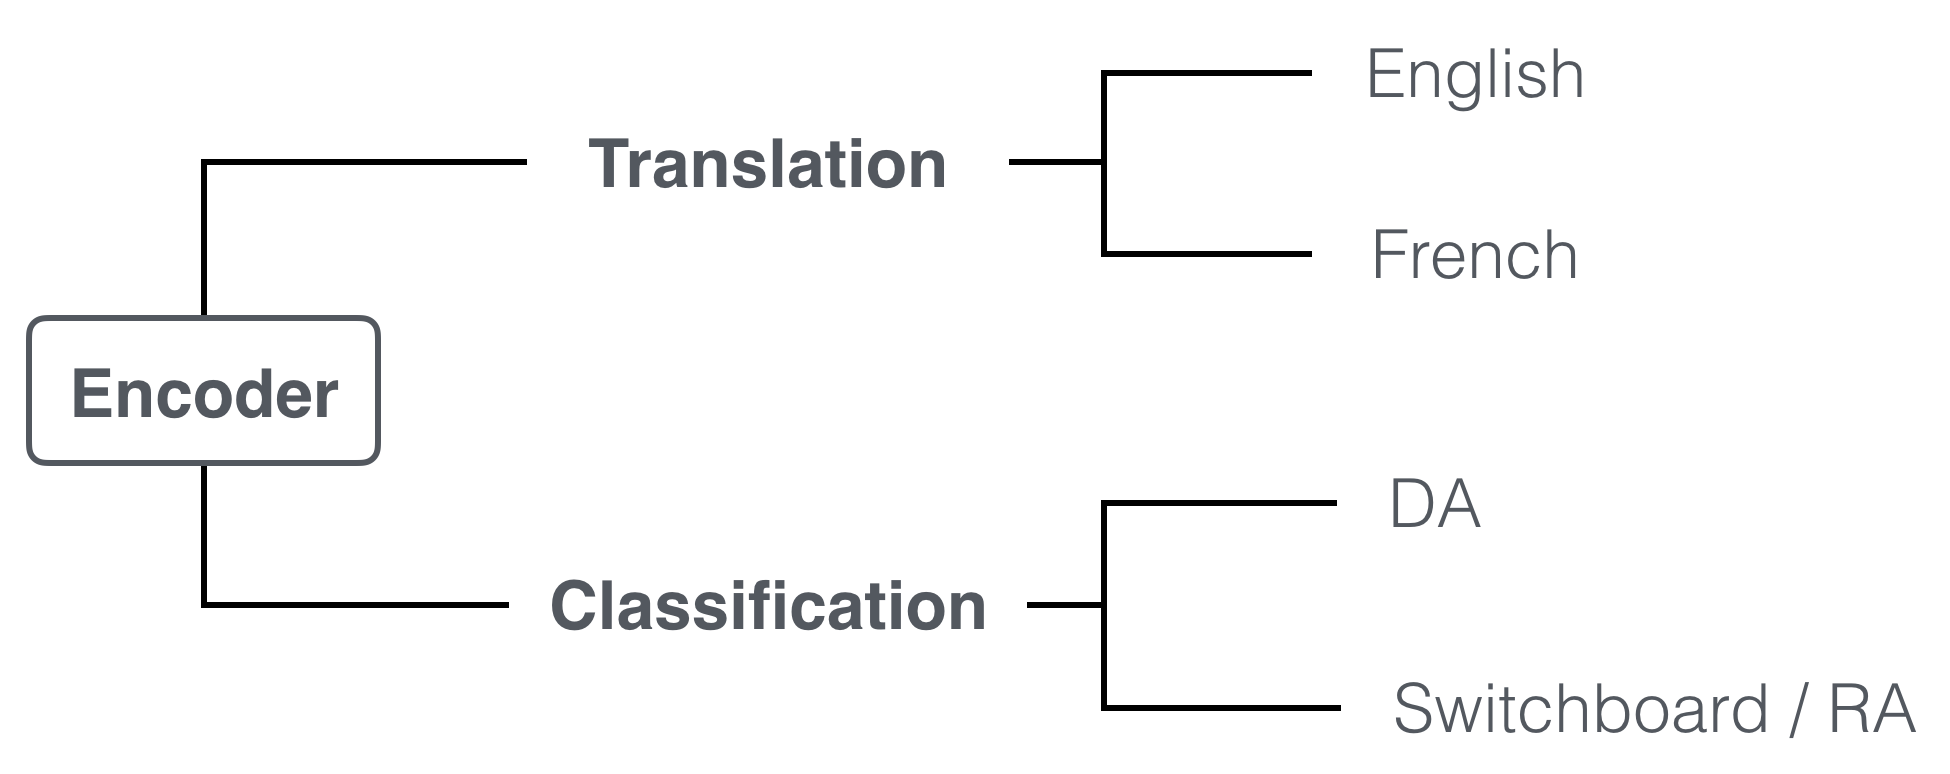
\includegraphics[scale=0.3]{summary.png}
\end{figure}


\end{frame}



















\section{Discussion}



%\subsection{PDE approach of prediction problem}


\begin{frame}
\frametitle{Discussion}
Possible future directions:
\begin{itemize}
\item ensemble
\item try different classifier, for example SVM
\item use the mean of the hidden state instead of the last state
\item add more features 
\end{itemize}


\end{frame}

\begin{frame}
\frametitle{Discussion: how much data do we need?}
It is difficult to predict the learning curve
\begin{itemize}
\item VC dimension provides a theoretical bound, which is useless in this case.
\item Depends on a lot of factors:
\begin{itemize}
\item classification method
\item complexity of the classifier
\item how well the classes are separated
\item data quality
\item \ldots
\end{itemize}
\end{itemize}

\end{frame}

\begin{frame}
\frametitle{Dataset used by LeCun et al. (Character-based ConvNet) }
\begin{figure}
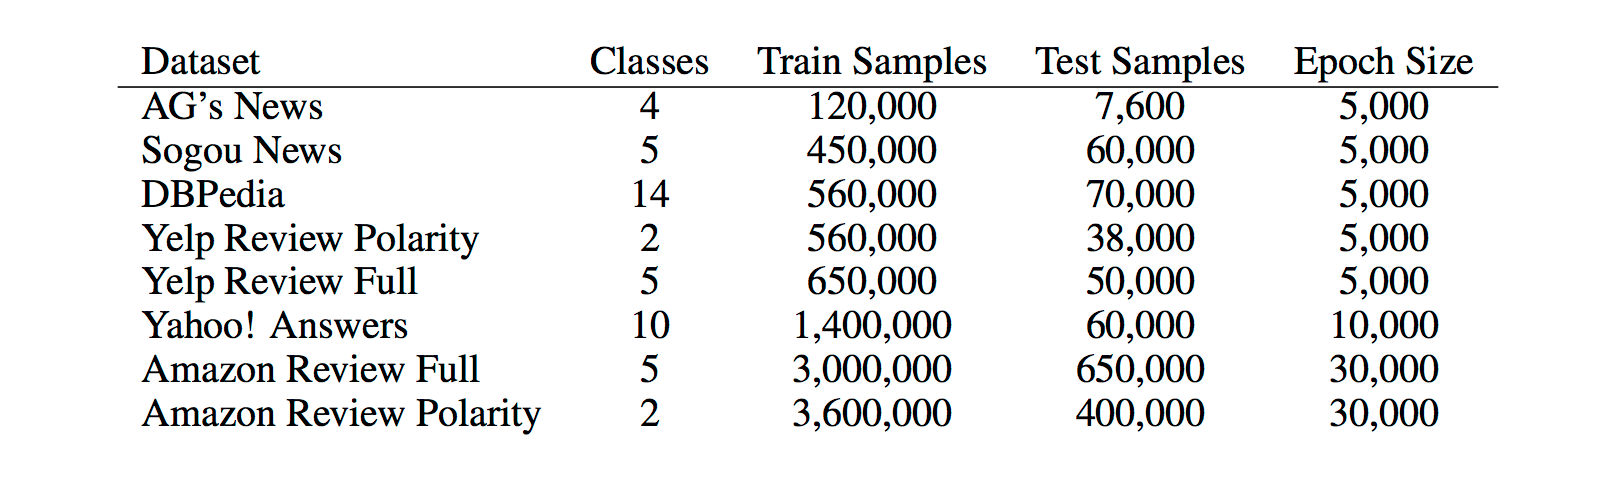
\includegraphics[scale=0.4]{conv_data}
\end{figure}

\end{frame}


\begin{frame}
\frametitle{Error Rate}
\begin{figure}
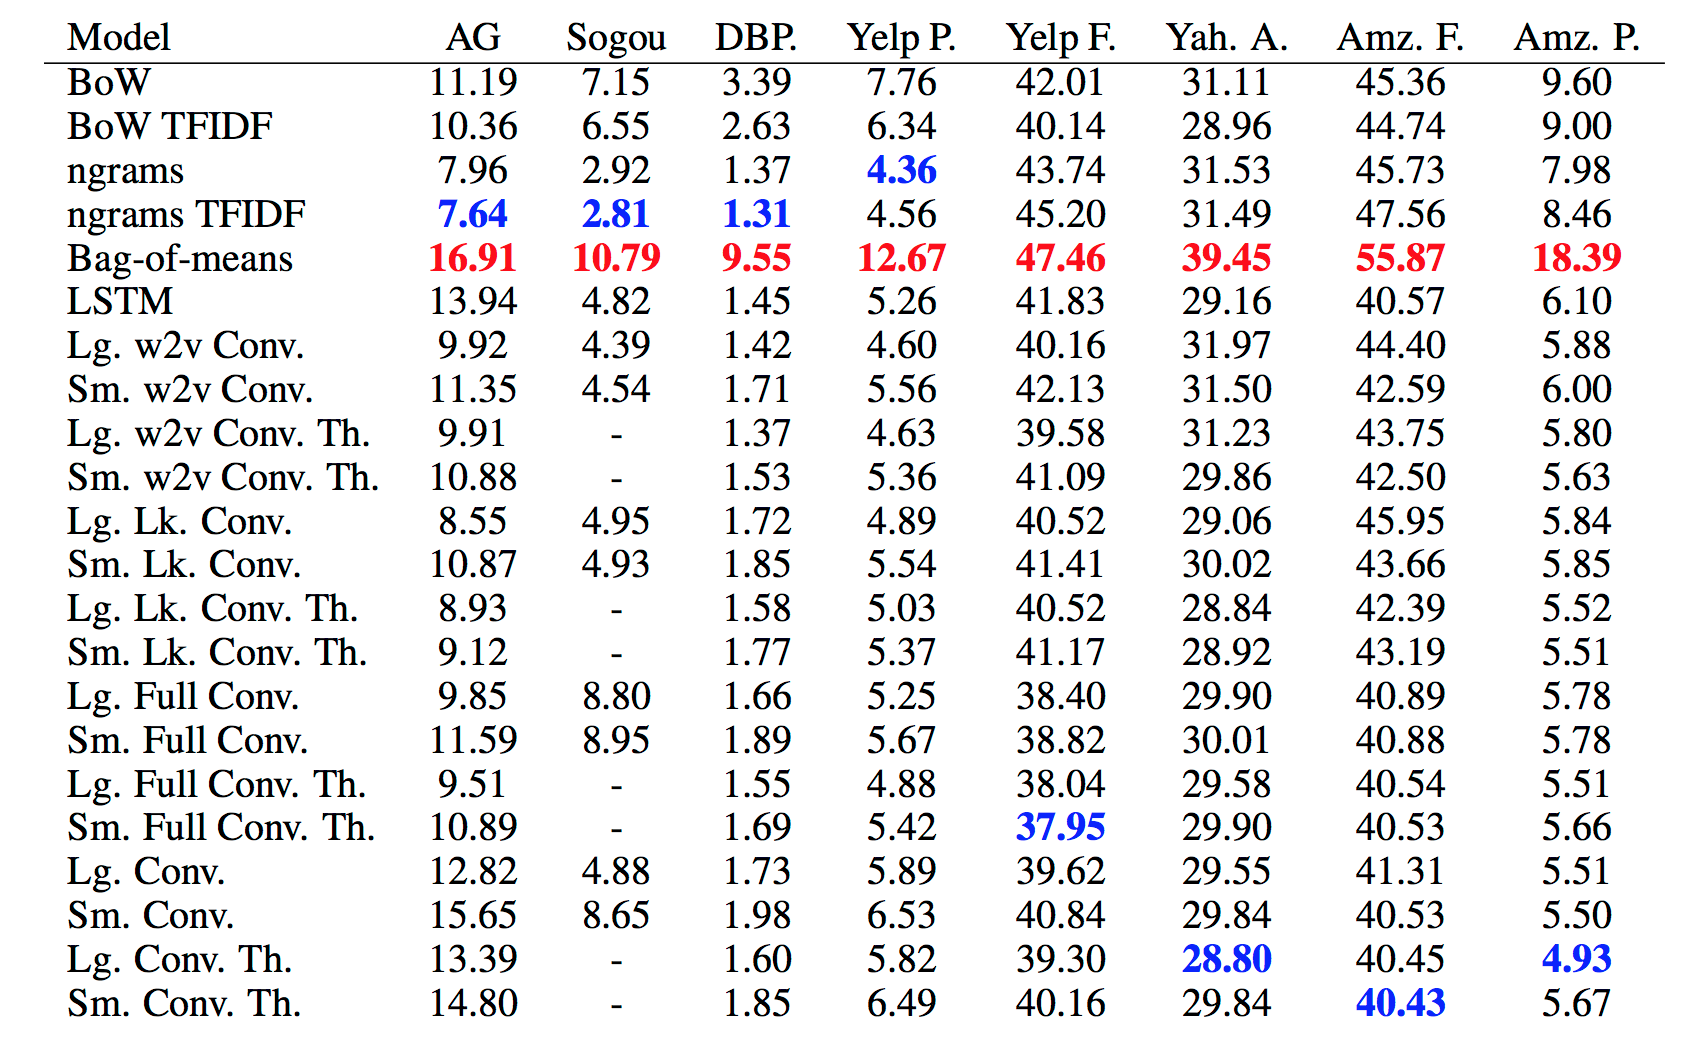
\includegraphics[scale=0.3]{error_rate}
\end{figure}
\end{frame}






\begin{frame}
\center
\huge Thank you.

\end{frame}




\end{document}